
\documentclass[8pt]{article}

\usepackage[utf8]{inputenc}

\usepackage{amsmath, bm}
\usepackage{graphicx}
\usepackage{amssymb}
\usepackage{float}
\usepackage{caption}
\usepackage{subcaption}
% set font size to 11pt

% set margin
\usepackage[margin=0.5in]{geometry}

\setlength{\parskip}{\baselineskip}%
\setlength{\parindent}{0pt}%
\setlength{\voffset}{-0.75in}
\setlength{\headsep}{5pt}

\begin{document}

% insert pdf cover page here

\title{Lab report: 3A3 Supersonic Nozzle}
\author{lwp26}
\date{October 2023}
\maketitle

\begin{abstract}
    \centering
    This report investigates supersonic flow ...
\end{abstract}

\section{Introduction}

Modern control systems

\section{Theory}

\subsection{Shocks}


\subsection{Boundary layers}


\subsection{Aims}

\begin{itemize}
\item To determine the 
\end{itemize}

\section{Results}

\newpage

\begin{figure}
    \centering
    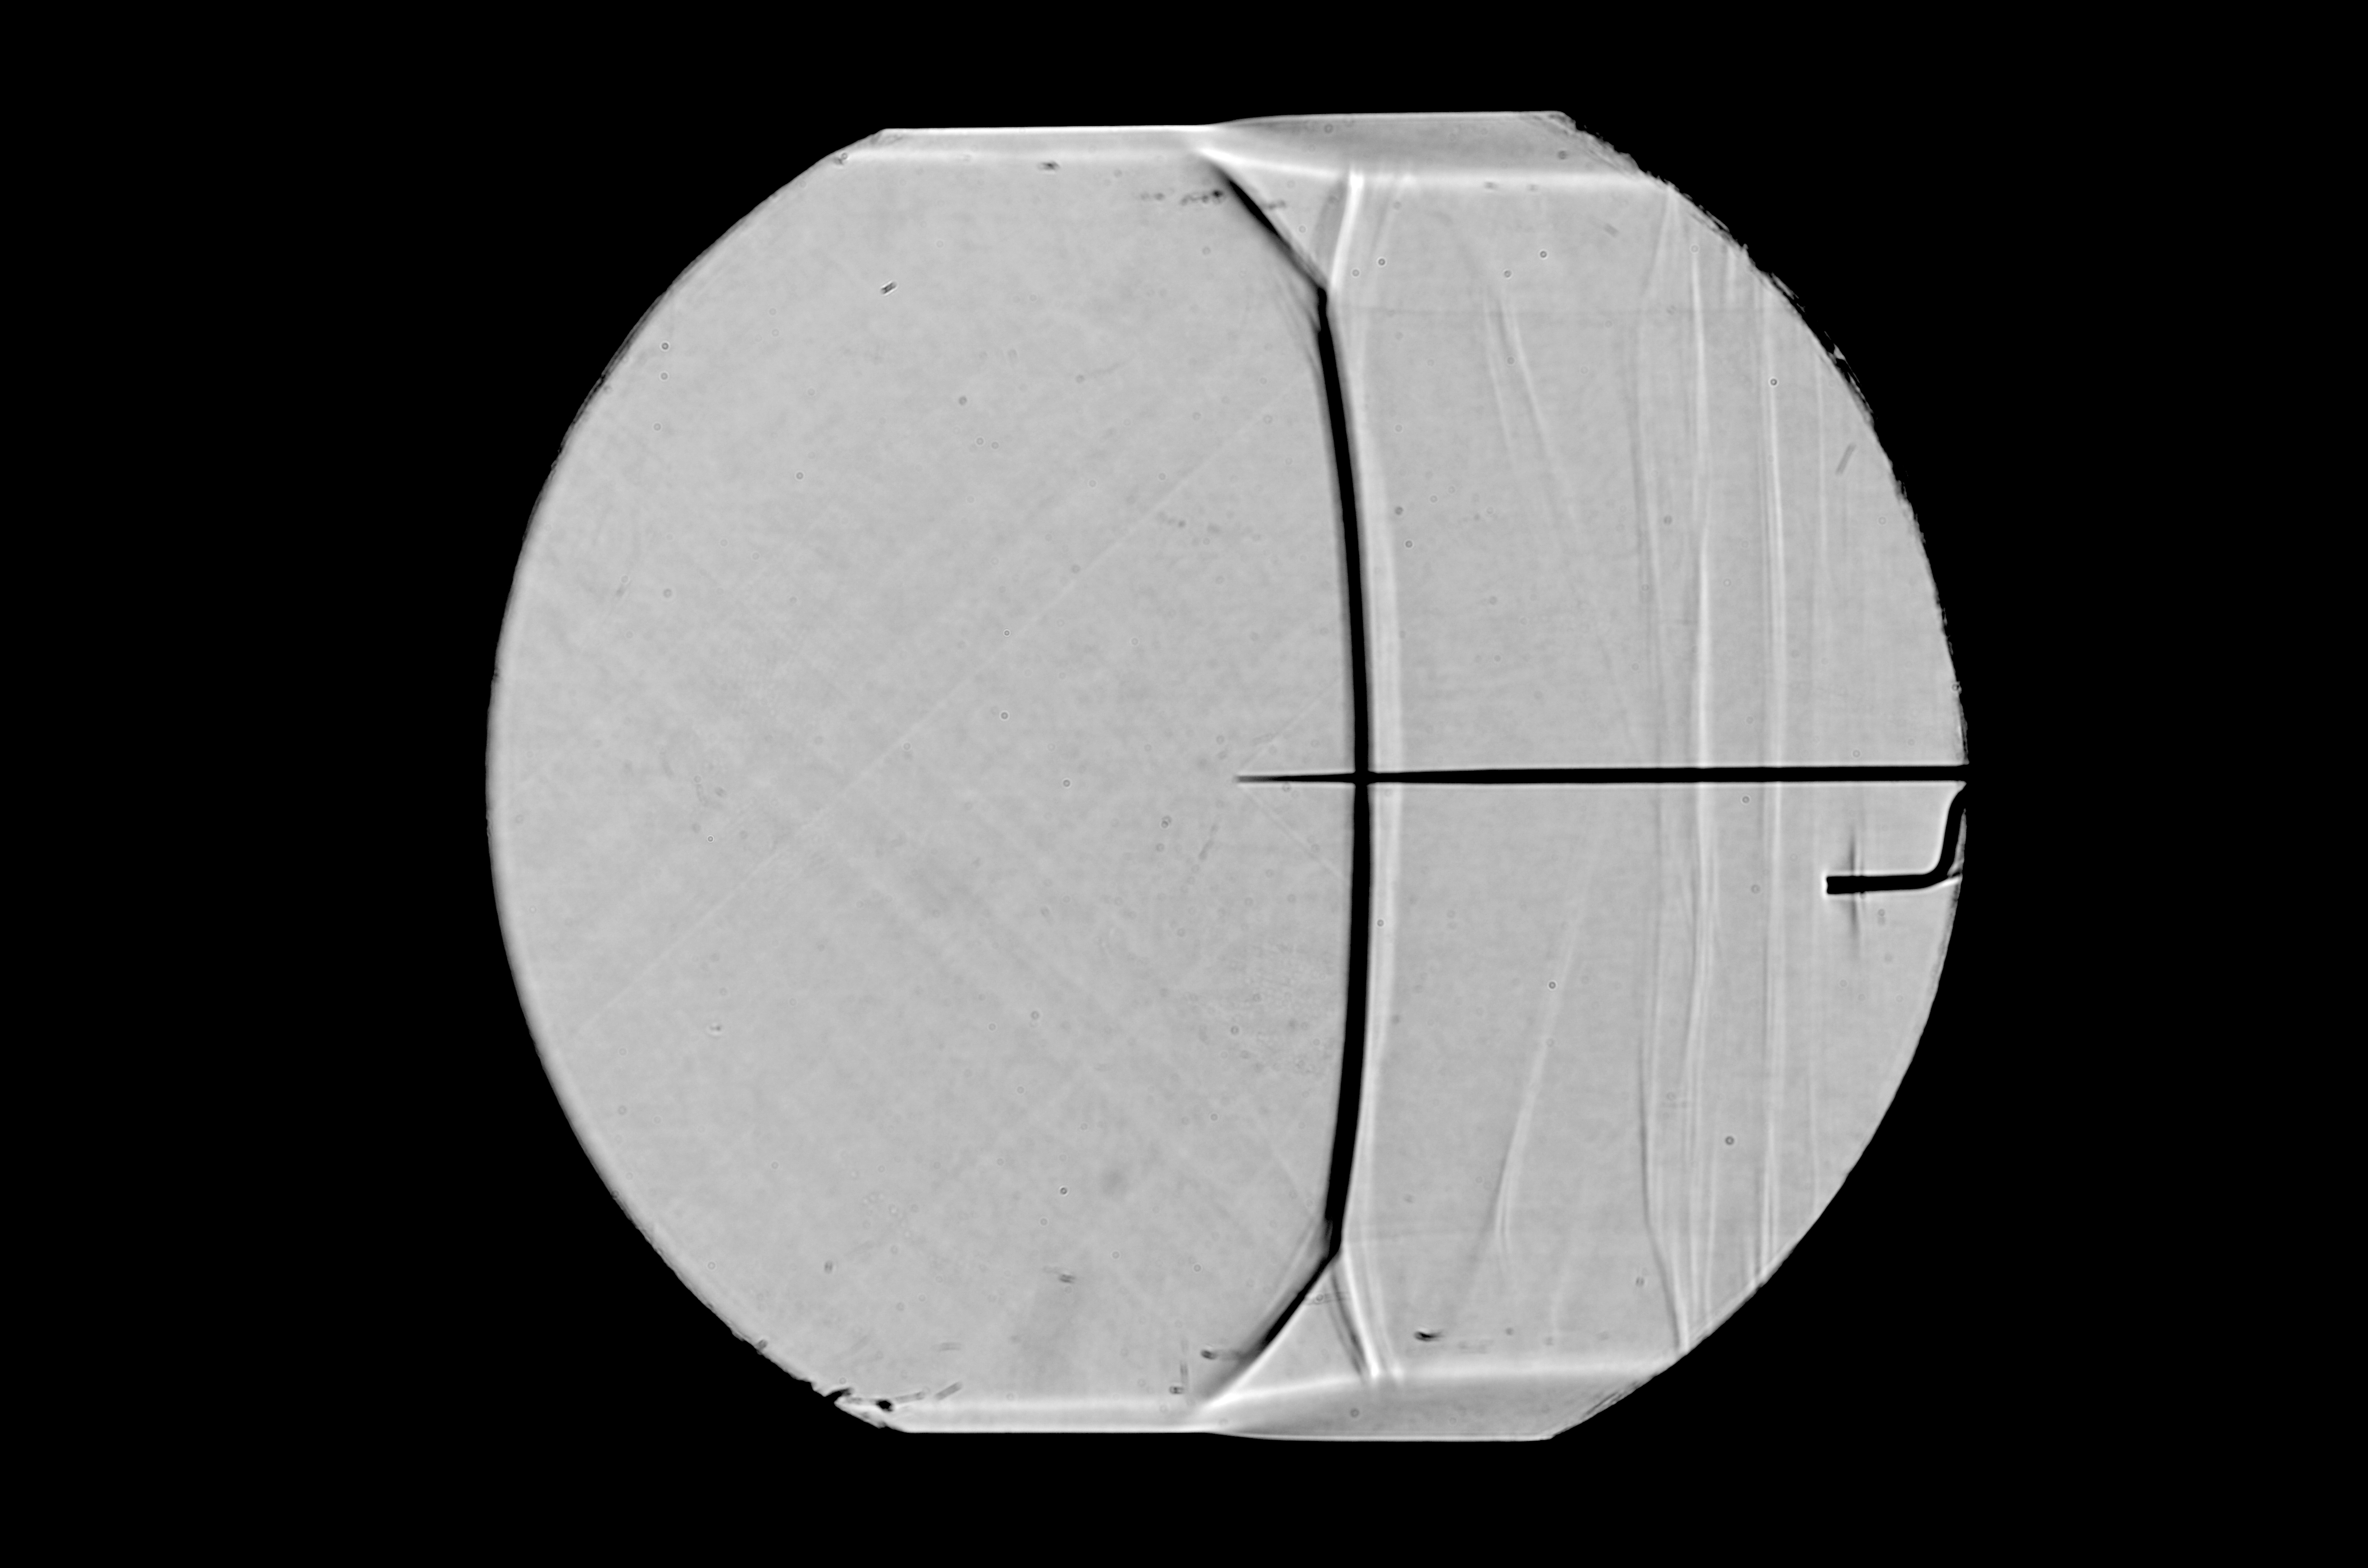
\includegraphics[width=0.8\textwidth]{starting_shock.jpg}
    \caption{Figure 1}
    \label{fig:figure1}
\end{figure}

\begin{figure}
    \centering
    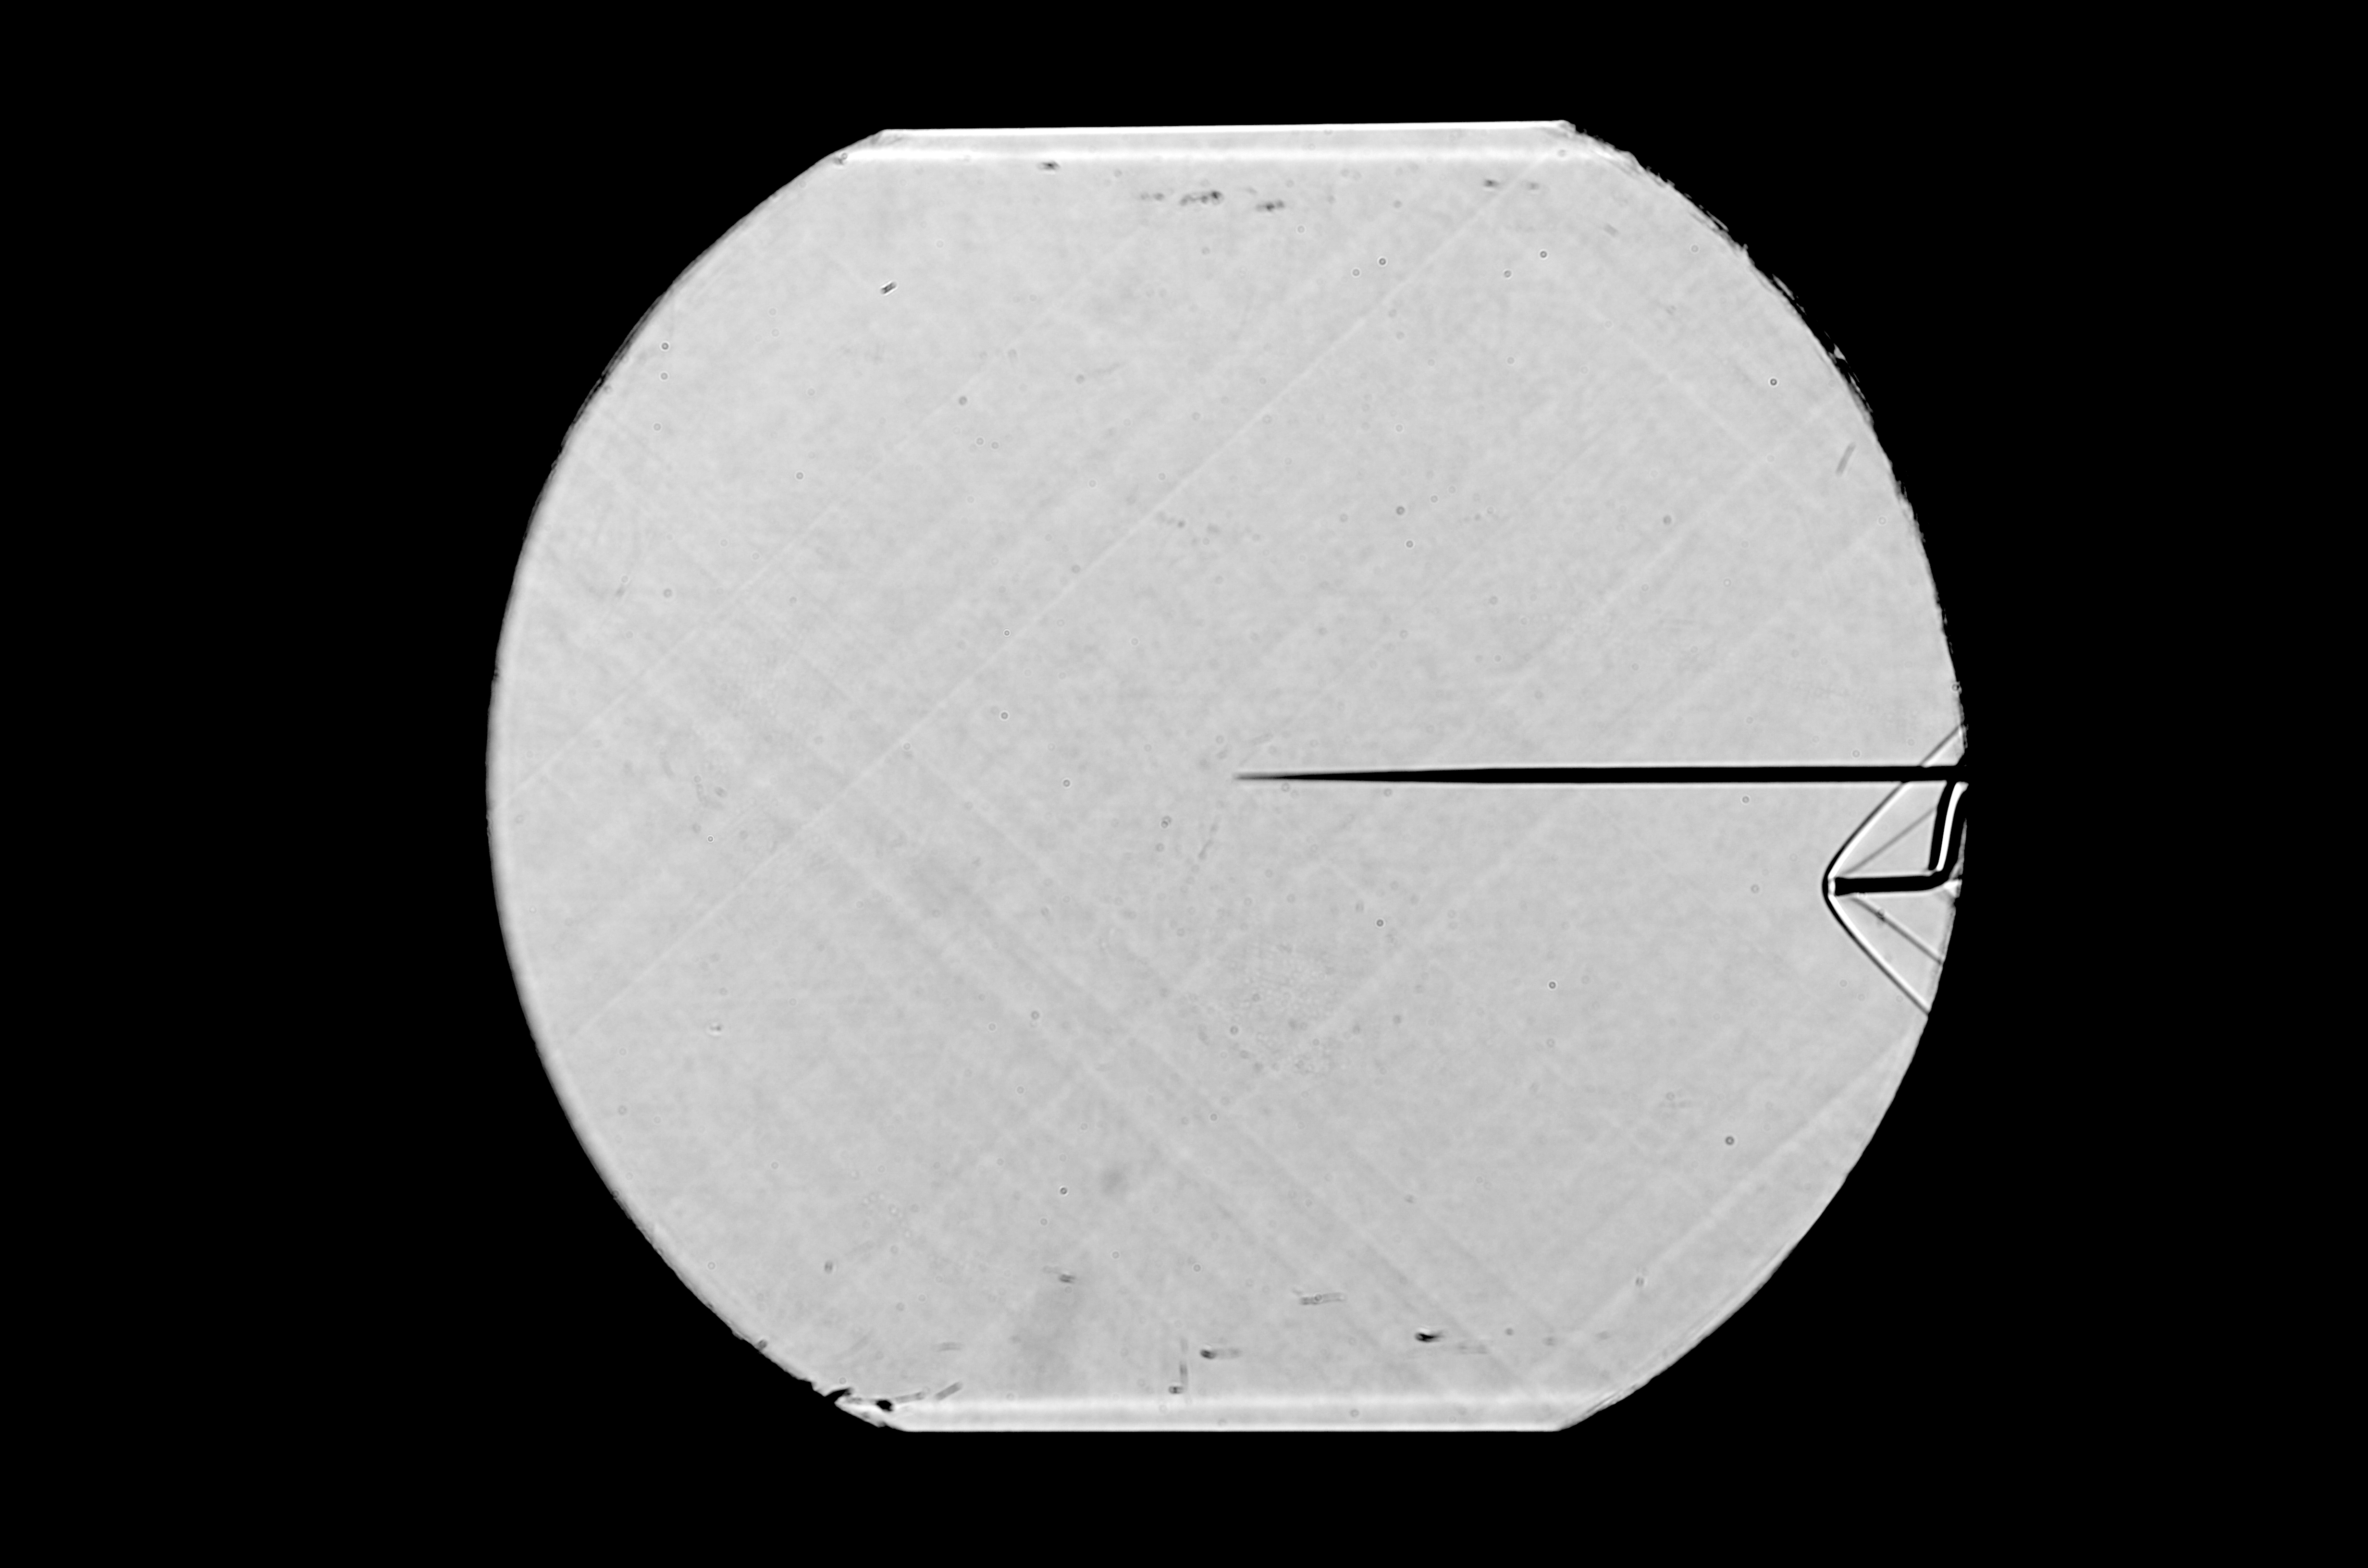
\includegraphics[width=0.8\textwidth]{working_state.jpg}
    \caption{Figure 2}
    \label{fig:figure2}
\end{figure}

\newpage

\begin{figure}
    \centering
    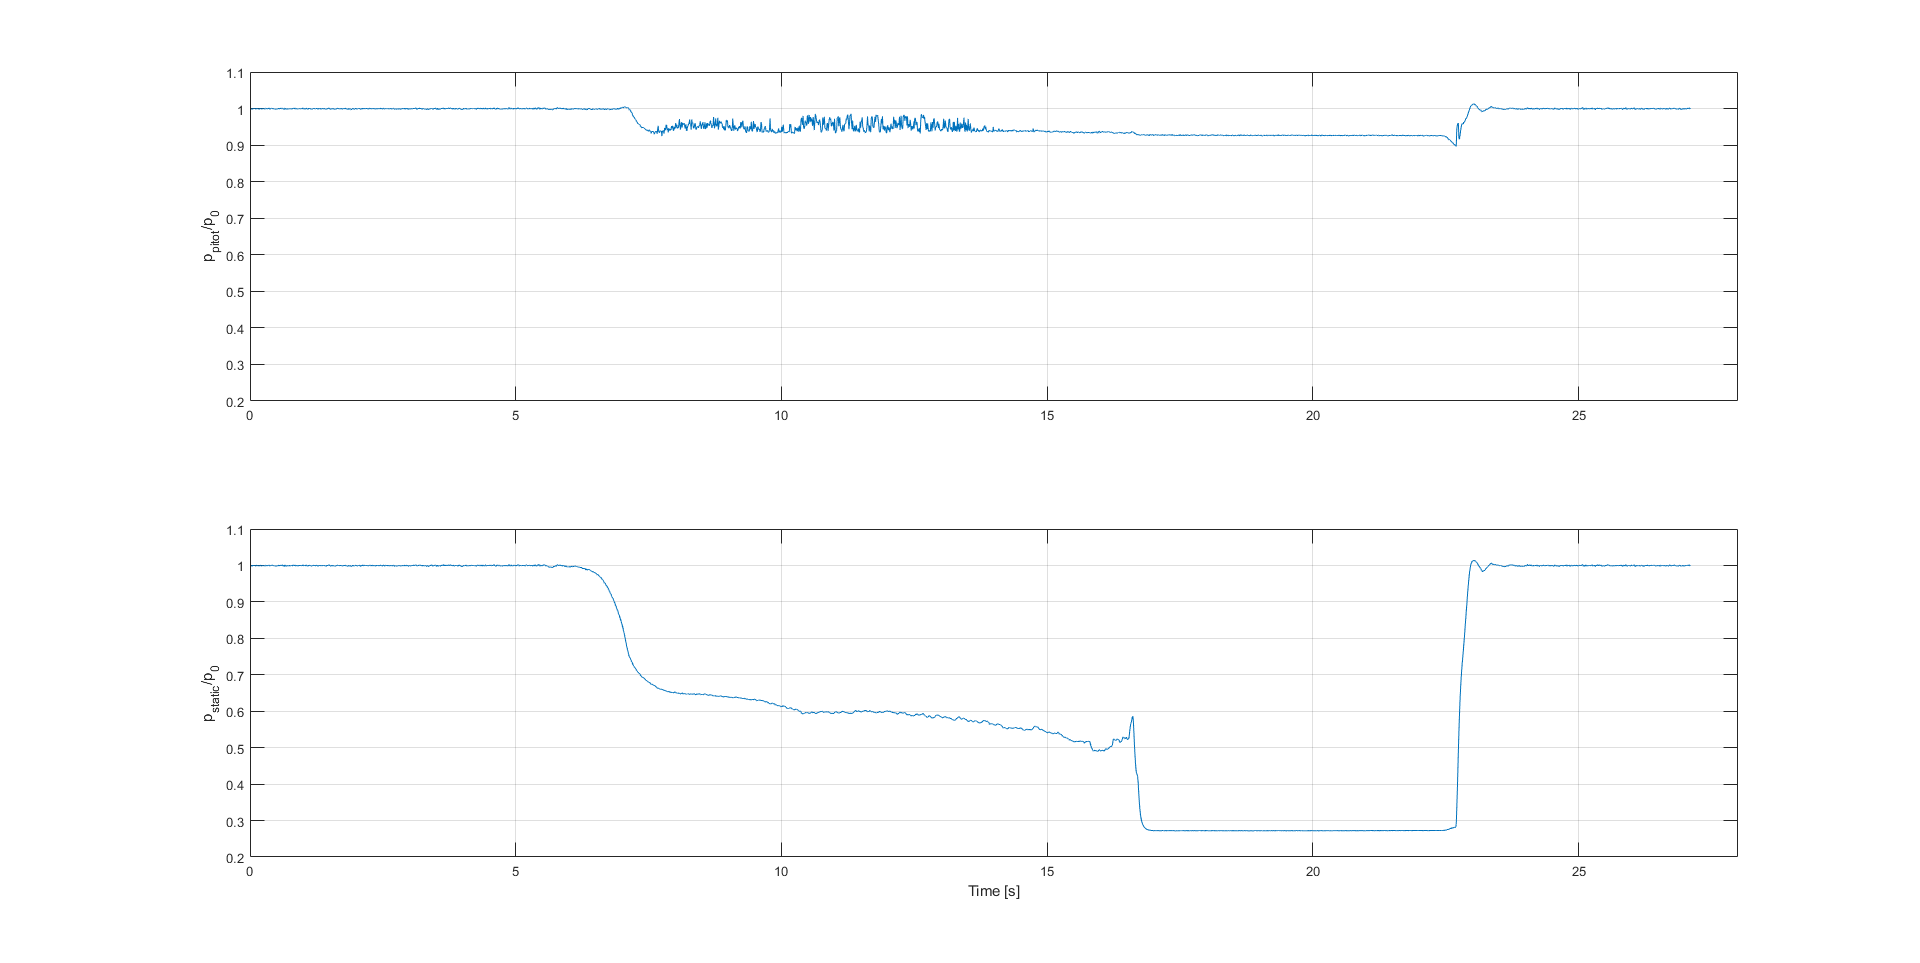
\includegraphics[width=0.8\textwidth]{tunnel_pressures.png}
    \caption{Figure 3}
    \label{fig:figure3}
\end{figure}

\newpage

\section{Discussion}

%interpret results and comment on anomalies

\subsection{Improvements}

\section{Conclusion}

From the experiments performed it can be observed that blah blah blah

\end{document}
